% !TeX program = xelatex
% !TeX encoding = UTF-8
%  请使用xeLaTeX进行编译
\documentclass[twoside,AutoFakeBold=true]{lixinthesis}  
%      onesid|twoside         postdoc 请选单栏(编写规则要求单面)


%%% 引用格式使用数字  [1,2] 
%\usepackage[numbers,comma, sort&compress]{natbib}      

%%% 引用格式使用上标  ^{[1,2]}
\usepackage[super,square,comma,sort&compress]{natbib} 

%%%使用GBT7714标准的参考文献格式 (按引用顺序排列参考文献)
\bibliographystyle{lixin-bachelor-check} 

%%%使用GBT7714标准的参考文献格式(按作者-日期排列参考文献)
%\bibliographystyle{gbt-author-year} 

%\usepackage{hypernat} 

\usepackage{empheq}
\usepackage{subfig,xcolor,color}
\usepackage{comment,multirow,float,zhlipsum,booktabs,tabularx}
\usepackage{tcolorbox,listings,matlab-prettifier}
\usepackage{float,subfig}

\tcbuselibrary{listings,breakable,skins}
%\lstset{
%	style = Matlab-editor,
%%	numbers = left,
%%	frame = single,
%}


\definecolor{dkgreen}{rgb}{0,0.6,0}
\definecolor{gray}{rgb}{0.5,0.5,0.5}
\definecolor{mauve}{rgb}{0.58,0,0.82}
\lstset{frame=none,
	aboveskip=3mm,
	belowskip=3mm,
	showstringspaces=false,
	columns=flexible,
	basicstyle={\small\ttfamily},
	numbers=none,
	numberstyle=\tiny\color{gray},
	keywordstyle=\color{blue},
	commentstyle=\color{dkgreen},
	stringstyle=\color{mauve},
	breaklines=true,
	breakatwhitespace=true,
	tabsize=4
}

\renewcommand{\lstlistingname}{代码}
% tcolorbox settings
\newtcolorbox{mybox}[1][]{fonttitle=\bfseries,title={#1}}
\newtcblisting{myexample}[1]{fonttitle=\bfseries,title=#1,listing and text}
\newtcblisting{myexample2}[1]{fonttitle=\bfseries,title=#1,listing side text}
\newtcblisting{listonly}[1]{fonttitle=\bfseries,title=#1,listing only}
% set search path
\graphicspath{{pic/}}

%%%    中文题名页
\title{一个立信非官方本科毕业论文\LaTeX 模板}
\englishtitle{An unofficial undergraduate\\ thesis \LaTeX~ template for LiXin}
\IDnumber{20201234}
\author{sslchi}
\school{统计与数学学院}
\major{数学与应用数学}
\class{2020级数学与应用数学1班}
\advisor{指导老师}
\submityear{\the\year{}}%提交年份
\submitmonth{\the\month{}}%提交月份
\submitday{\the\month{}} %提交日
\makesignature % 如需要手写签名,将本行注释去掉


%%%%%%%%%%%%%%%%%% 自定义宏命令 %%%%%%%%%%%%%%%

\renewcommand{\d}{\mathrm{d}} %% \d 已经有\d 这个命令,用renewcommand
\newcommand{\dx}{\mathrm{d}x} %% \dx 没有\dx 这个命令,用newcommand

%%%%%%%%%%%%%%%%%%%


\begin{document}


\maketitle  %%%% 制作封面


\frontmatter %%%% 前文部分

\begin{abstract}
	
本文简要介绍了本科毕业论文\LaTeX 模板的使用方法。在此,模板作者作声明如下:
\begin{enumerate}
    \item 本模板为作者无偿制作撰写,任何人都可以免费使用本模板。
    \item 本模板未经学校相关部门审核及授权,在使用前请务必斟酌。
    \item 作者不对模板能够通过学校/学院的格式审查做任何明示或暗示的保证,任何由于使用本模板而引起的论文格式审查问题均与本模板作者无关。	
\end{enumerate}


\keywords{毕业论文; \LaTeX 模板。}


\end{abstract}

\begin{englishabstract}

This article briefly introduces the usage of the undergraduate  \LaTeX~ thesis template. The template author makes the following statements:
\begin{enumerate}
    \item This template was created and written by the author voluntarily, and anyone can use it for free.
    \item This template has not been reviewed or authorized by the relevant school departments, so please carefully consider its use.
    \item The author makes no explicit or implicit guarantees that the template will pass the school/college's format review. Any issues arising from the use of this template concerning the format review are not the responsibility of the template author.
\end{enumerate}


\englishkeywords{\LaTeX\ Templates; thesis.}

\end{englishabstract}



\tableofcontents


\mainmatter %%%% 正文部分

\section{免责声明(Disclaimer)}
本文简要介绍了本科毕业论文\LaTeX 模板的使用方法。在此,模板作者作声明如下:
\begin{enumerate}
	\item 本模板为作者无偿制作撰写,任何人都可以免费使用本模板。
	\item 本模板未经学校相关部门审核及授权,在使用前请务必斟酌。
	\item 作者不对模板能够通过学校/学院的格式审查做任何明示或暗示的保证,任何由于使用本模板而引起的论文格式审查问题均与本模板作者无关。	
\end{enumerate}

This article briefly introduces the usage of the undergraduate  \LaTeX~ thesis template. The template author makes the following statements:
\begin{enumerate}
    \item This template was created and written by the author voluntarily, and anyone can use it for free.
    \item This template has not been reviewed or authorized by the relevant school departments, so please carefully consider its use.
    \item The author makes no explicit or implicit guarantees that the template will pass the school/college's format review. Any issues arising from the use of this template concerning the format review are not the responsibility of the template author.
\end{enumerate}

\section{系统要求}
模板通过 CTeX 宏包来获得中文支持。 CTeX 宏包提供了一个
统一的中文\LaTeX 文档框架, 一般情况下,在安装TeXLive或其它发行版时,它已经被下载,无需单独下载。

此外, 模板还使用了 amsmath、 amsthm、 amsfonts、amssymb、 bm 和 hyperref等宏包。

\subsection{下载与安装}
模板的最新版本可以从\url{https://github.com/sslchi/lixinthesis}下载。模板包含一个文档类型文件.cls以及一个使用模板文件main.tex(也即本文的源文件),用户
可以通过修改这个main.tex以及chap文件夹下的内容撰写自己的学位论文。


由于参考文献使用GB7714标准,因此文档中还包含了Zeping Lee(李泽平) 编写的参考文献的样式文件(即两个后缀为.bst的文件,项目链接为:\url{https://github.com/zepinglee/gbt7714-bibtex-style})。

\subsection{编译方式}
本模板基于cetxart宏包,暂时只支持xeLaTeX方式进行编译。使用{\bfseries TexStudio编辑器}的用户可以直接点击编辑器上的构建并查看按钮进行编译,无需进行设置; 使用其它编辑器的用户请设置编译方式为xeLaTeX。 {\color{red}目前,只在TeXLive 2023、2024上测试过,如果不能运行,请先检查版本是否是TeXLive 2023、2024。}

\subsection{常见问题}

\begin{enumerate}
    \item 如提示缺少字体,请下载相应的字体。
    \item 如中文显示乱码, 请检查文件的编码方式,并将编码方式设置为utf8。
    \item 使用在线\LaTeX~编辑器overleaf时,因其所用系统为Ubuntu,字体与Win系统下的字体略有差别。
\end{enumerate}

\subsection{问题反馈}
因为毕业论文的要求很详细,从字体到到段距、行距等,细节不知凡几。因此难免有疏漏之处{\color{red}(再次申明,作者不对模板能够通过学校/学院的格式审查做任何明示或暗示的保证)},因此用户在使用中如果发现问题,可以联系:
\begin{center}
公众号:MathICU
\end{center}

{\large \color{red}如果有同学愿意接手这个模板的维护,那是再好不过的了。}



\section{基本选项及命令介绍}\label{sec:basic}
本节介绍模板的一些基本选项和命令。



\subsection{模板中的选项及命令}
封面上的所有信息可以通过下列带参数的命令进行修改。
\begin{mybox}
\begin{tabular}{p{10cm}p{5cm}}
	\verb|\title|         & 标题\\
	\verb|\englishtitle|  & 英文标题\\
	\verb|\IDnumber|      & 学号\\
	\verb|\author|        & 作者\\
	\verb|\school|        & 学院\\
	\verb|\major|         & 专业\\
	\verb|\class|         & 班级\\ 
	\verb|\submityear|    & 提交年\\
	\verb|\submitmonth|   & 提交月\\
    \verb|\submitday|     & 提交日(声明页签名日)\\
\end{tabular}
\end{mybox}
\noindent 例如,本文的中文标题为“一个立信非官方本科毕业论文\LaTeX 模板”,可以使用命令
\begin{listonly}{}
\title{一个立信非官方本科毕业论文\LaTeX 模板}
\end{listonly}
\noindent 获得。

\subsection{手写签名}
如果需要手写签名,在导言区(\verb|\begin{document}|之前)加上\verb|\makesignature|命令,并将pic文件夹下的signature改成自己的手写签名即可更新声明页中的签名。注意制作手写签名时,应使签名居中,且签名四周要留些许空白(但不要过多)。


\subsection{各级标题}
各级标可以使用如下命令获得:
\begin{mybox}
	\begin{tabular}{p{10cm}p{5cm}}
		\verb|\section|         	& 一级标题\\
		\verb|\subsection|       	& 二级标题\\
		\verb|\subsubsection|      	& 三级标题\\
		\verb|\paragraph|        	& 四级标题\\
	\end{tabular}
\end{mybox}
\noindent 例如,下面是一个三级标题的使用示例:
\begin{myexample}{使用标题示例}
\subsubsection{这是一个三级标题}
\end{myexample}
\noindent 其它级别的标题类似。


\subsection{定理环境}
在模板中,我们还预先定义了一些定理环境。这些环境的名字及意义如下
\begin{mybox}
	\begin{tabular}{p{10cm}p{5cm}}
		\verb|example|         	& 例\\
		\verb|theorem|       	& 定理\\
		\verb|remark|      		& 注\\
		\verb|lemma|        	& 引理\\
		\verb|definition|       & 定义\\
		\verb|proof|         	& 证明\\
	\end{tabular}
\end{mybox}
\noindent 使用方法如下:
\begin{myexample}{定理环境使用举例}
\begin{definition}[直角三角形]\label{def:exm1}
    若三角形有一个角是直角,则称该三角形为直角三角形。
\end{definition}
可以使用定理~\ref{def:exm1}引用该定理。
\end{myexample}
\noindent 其余定理环境的使用方式类似。
\section{\LaTeX 基本用法}
本节介绍\LaTeX 的基本用法。关于\LaTeX 更详细的介绍,读者可以自行阅读\LaTeX~的相关教材,如刘海洋老师的《LaTeX入门》\cite{Liu2013}。

\subsection{数学公式}
数学公式易学难精,如果比较考究,需要注意的事项非常多。下面的例子里面,上面或者左边是在\LaTeX~文档中输入的代码,下面或者右边是编译之后输出的内容\footnote{这样可以得到一个脚注。}。

\subsubsection{基本用法}
数学公式分行内公式和行间公式。下面的例子说明了如何使用行内公式和行间公式,其中,上半部分是LaTeX中的内容,下半部分是输出。


将字母置于两个美元符号之间,即可得到一个行内公式,下面是一个简单的行内公式举例:
\begin{myexample2}{行内公式}
这是一个行内公式$a^2+b^2=c^2$。
\end{myexample2}

如果公式两边各有两个美元符号,可以得到一个不带编号的行间公式,需要注意的是行间公式应该看成句子的一部分,因此大部分情况需要在行间公式添加标点符号。下面是一个简单的行间公式的例子:
\begin{myexample}{不带编号的行间公式}
这里是一个行间公式
$$a^2+b^2=c^2,$$
其中$a$和$b$是直角边的长度,$c$是斜边的长度。
\end{myexample}

下面介绍一些常用的公式书写方式:
\begin{enumerate}
\item 这是上标下标
$$a_1,\ a_2,\ \ldots,\ a_n, \ x^2,\ x^{n+1},\ \mathrm{e}^{i\pi} + 1 = 0;$$

\item 这是求和,积分,求极限
$$\sum_{i=1}^n i = \frac{n(n+1)}{2}, \
\int_0^1 x^2\, dx = \frac{1}{3},\
\lim_{x \to 0} \frac{\sin x}{x} = 1;$$

\item  这是特殊符号
$$\infty,\ \partial,\ \nabla,\ \alpha,\ \beta,\ \gamma,\ \ldots;$$

\item 这是分数
$$\frac{a}{b+c},\ \frac{a}{b+\frac{c}{d}};$$

\item 这是矩阵、行列式
$$
A = \begin{bmatrix}
1 & 2 & 3 \\
4 & 5 & 6 \\
7 & 8 & 9
\end{bmatrix},\ 
B = \begin{pmatrix}
1 & 2 & 3 \\
4 & 5 & 6 \\
7 & 8 & 9
\end{pmatrix},\ 
C = \begin{vmatrix}
1 & 2 & 3 \\
4 & 5 & 6 \\
7 & 8 & 9
\end{vmatrix},\ 
D = \begin{Vmatrix}
1 & 2 & 3 \\
4 & 5 & 6 \\
7 & 8 & 9
\end{Vmatrix}.
$$

\end{enumerate}


如果想得到一个带编号的行间公式,可以使用公式环境,下面是一个带编号的行间公式:
\begin{myexample}{带编号的行间公式}
这里是一个带编号的行间公式
\begin{equation}\label{eq:exm1}
    a^2+b^2=c^2.
\end{equation}
\end{myexample}

公式环境中的\verb|\label|命令后的参数,可以让我们方便地进行公式引用,如果不需要引用,则不必添加label。。
你可以使用合适的字母为公式命名,并使用\verb|\eqref{}|进行引用。下面是一个公式引用的例子:
\begin{myexample}{公式引用}
在这里,我们可以使用\eqref{eq:exm1}引用上述公式。
\end{myexample}

在LaTeX中,章节、图、表、定理等的引用与公式的引用类似,只需在相应位置加上\verb|\label{标签}| 即可引用,需要注意的是,其余引用,使用\verb|\ref{标签}|即可。注意,公式引用使用的是\verb|\eqref{}|,它可以在编号两侧自动加上括号。


如果公式太长,可以使用split环境进行换行,下面是一个公式换行的例子:
\begin{myexample2}{公式换行}
\begin{equation}
    \begin{split}
        a+b+c &= c+d+e \\
              &+ f+g+h.
    \end{split}
\end{equation}
\end{myexample2}
\noindent 注意,在上面的例子中,我们使用\&让等号和加号对齐。

如果需要使用方程组,可以使用以下几种方式得到:
\begin{myexample2}{使用cases环境}
\begin{equation}
    \begin{cases}
        x + y &= 1, \\ % & 用来对齐
        x - y &= 2.
    \end{cases}
\end{equation}
\end{myexample2}

\begin{myexample2}{使用aligned环境}
\begin{equation}
\left\{
    \begin{aligned}
        x + y &= 1, \\ %& 用来对齐
        x - y &= 2.
    \end{aligned}
\right.
\end{equation}
\end{myexample2}


\begin{myexample2}{使用align环境}
\begin{align}
    x + y &= 1, \\ %& 用来对齐
    x - y &= 2.
\end{align} 
\end{myexample2}

\begin{myexample2}{使用eqnarray环境}
\begin{eqnarray}
    x + y &= 1, \\ %& 用来对齐
    x - y &= 2.
\end{eqnarray} 
\end{myexample2}

如果需要带大括号且每个方程都有编号的公式,则需要使用其它宏包,如empheq,的支持。
\begin{myexample}{使用其它宏包}
\begin{empheq}[left=\empheqlbrace]{align}
    x + y &= 1, \\
    x - y &= 2, \\
    2x + 3y &= 5.
\end{empheq}
\end{myexample}



\subsubsection{特别注意事项}
值得注意的是,在数学公式环境中,有些符号应该使用直体,例如:
\begin{enumerate}
	\item 微分符号$d$应该用直体,写作$\d x$;
	\item $max$应写作$\max$, $min$应写作$\min$;
	\item 三角函数应写作直体,如$sin$应写作$\sin$;
	\item 英文缩写等应写成直体,如$\mathrm{s.t.}$;
    \item 公式中包含的单词,应写成直体,如$\mathrm{for}$。
\end{enumerate}
在公式环境中,使用{\ttfamily $\backslash$mathrm\{\}}可以获得直体字母,示例如下:
\begin{myexample}{}
$a^2+b^2=c^2,\ \mathrm{for}\ a>0$. %可以用\ 表示空格
\end{myexample}

\subsection{图形和表格}\label{sec:tabfig}

我们可以使用figure环境和table环境插入图片和表格。

\begin{listonly}{图形示例}
\begin{figure}[htbp]
    \begin{center}
        
\includegraphics[width=0.35\linewidth]{lixinlogo.jpg}\quad
        
\includegraphics[width=0.35\linewidth]{lixinlogo.jpg}
    \end{center}
    \caption[图形示例]{两个校徽}\label{fig:exm1}
\end{figure}
\noindent 可以使用图~\ref{fig:exm1}引用该图片。% \noindent 表示该行不缩进
\end{listonly}

\noindent 上述内容可以得到如下输出:
\begin{figure}[htbp]
	\begin{center}
		
\includegraphics[width=0.35\linewidth]{lixinlogo.png}\quad
		
\includegraphics[width=0.35\linewidth]{lixinlogo.png}\\
            
\includegraphics[width=0.35\linewidth]{lixinlogo.png}\quad
		
\includegraphics[width=0.35\linewidth]{lixinlogo.png}
	\end{center}
	\caption{四个校徽}\label{fig:exm1}
\end{figure}

\noindent 可以使用图~\ref{fig:exm1}引用该图片。% \noindent 表示改行不缩进


如果想让一个图中的每个小图都有小标题,则可以使用subfig宏包中的subfloat环境,下面是一个这种例子。
\begin{figure}[htbp]    
  \centering            
  \subfloat[第一个子图标题]   
  {
\includegraphics[width=0.35\linewidth]{lixinlogo.png} \label{fig:subfig1}}\quad
  \subfloat[第二个子图标题]
  {
\includegraphics[width=0.35\linewidth]{lixinlogo.png} \label{fig:subfig2}}\\
  \subfloat[第三个子图标题]   
  {
\includegraphics[width=0.35\linewidth]{lixinlogo.png} \label{fig:subfig3}}\quad
  \subfloat[第四个子图标题]
  {
\includegraphics[width=0.35\linewidth]{lixinlogo.png} \label{fig:subfig4}}\\
  \caption{四个校徽}    
  \label{fig:subfig}
\end{figure}

\noindent 子图也可以进行交叉引用,例如图~\ref{fig:subfig1}。


表格也是呈现数据或者数值结果的一个重要方式。在\LaTeX~中,我们一般使用table环境和tabular环境产生表格,下面是一个表格和表格引用的例子。
\begin{listonly}{表格示例}
\begin{table}[htbp]
    \caption{三线表}\label{tab:exp1}
    \begin{center}
        \newcolumntype{C}{>{\centering\arraybackslash}X}%
        \begin{tabularx}{0.9\linewidth}{CCCCCC}
            \toprule
            1 & 2 & 3 & 4 & 5 & 6\\
            \midrule
            1 & 2 & 3 & 4 & 5 & 6\\
            1 & 2 & 3 & 4 & 5 & 6\\
            1 & 2 & 3 & 4 & 5 & 6\\
            \bottomrule
        \end{tabularx}
    \end{center}
\end{table}
\noindent 可以使用表~\ref{tab:exm1}引用该表格。% \noindent 表示改行不缩进
\end{listonly}

\noindent 上述内容可以得到如下输出:


\begin{table}[htbp]
	\caption{三线表}\label{tab:exm1}
	\begin{center}
		\newcolumntype{C}{>{\centering\arraybackslash}X}%
		\begin{tabularx}{0.9\linewidth}{CCCCCC}
			\toprule
			1 & 2 & 3 & 4 & 5 & 6\\
			\midrule
			1 & 2 & 3 & 4 & 5 & 6\\
			1 & 2 & 3 & 4 & 5 & 6\\
			1 & 2 & 3 & 4 & 5 & 6\\
			\bottomrule
		\end{tabularx}
	\end{center}
\end{table}
\noindent 可以使用表~\ref{tab:exm1}引用该表格。% \noindent 表示改行不缩进

\subsection{代码抄录}
使用lstlisting环境可以进行代码抄录,本模板中的设置适用于Matlab, 用户也可以定制适合自己所用语言的设置。


\begin{myexample}{代码抄录环境示例}
\begin{lstlisting}[caption=代码抄录示例,language=Matlab,label=code:exm1]
function s = f(x)
% This Program gives the area of a circle.
% S = F(x)
    pi = 3.14;
    
    s = pi*x^2;
end
\end{lstlisting}
可以使用代码~\ref{code:exm1}引用代码。
\end{myexample}

\subsection{参考文献}

参考文献需要再bibref.bib中进行编写,如为图书,应像下方一样输入:
\begin{mybox}
\begin{lstlisting}
@book{Liu2013,
	title={LATEX入门},
	author={刘海洋},
	publisher={电子工业出版社},
	address = {北京},
	year={2013},
}
\end{lstlisting}	
\end{mybox}

\noindent 如为文章,则应像下方一样输入:
\begin{mybox}
\begin{lstlisting}
@article{Driscoll2024aaa,
	title={{AAA} rational approximation on a continuum},
	author={Driscoll, Tobin A and Nakatsukasa, Yuji and Trefethen, Lloyd N},
	journal={SIAM Journal on Scientific Computing},
	volume={46},
	number={2},
	pages={A929--A952},
	year={2024},
	publisher={SIAM}
}
\end{lstlisting}
\end{mybox}
注意上面标题中的AAA三个字母用大括号括起来了,如果不这样做,输出的参考文献会显示为Aaa.

\noindent 引用时,使用{\ttfamily$\backslash$cite\{\}}即可引用,例如:
\begin{myexample}{参考文献使用示例}
参考文献可以这样引用\cite{Liu2013}。
两篇或者多篇可以这样引用\cite{Liu2013,Driscoll2024aaa}。
\end{myexample}

\noindent 其它文献类型如下
\begin{mybox}
\begin{tabular}{p{4.5cm}p{2cm}p{6.5cm}}
文献类型         &  标识代码 &  Entry Type\\
\hline
普通图书         &  M        &  @book \\
图书的析出文献   &  M        &  @incollection\\
会议录           &  C        &  @proceedings\\
会议录的析出文献 &  C        &  @inproceedings 或 @conference\\
汇编             &  G        & \textcolor{red}{@collection}\\
报纸             &  N        & \textcolor{red}{@newspaper}\\
期刊的析出文献   &  J        &  @article\\
学位论文         &  D        &  @mastersthesis 或 @phdthesis\\
报告             &  R        &  @techreport\\
标准             &  S        &  \textcolor{red}{@standard}\\
专利             &  P        &  \textcolor{red}{@patent}\\
数据库           &  DB       &  \textcolor{red}{@database}\\
计算机程序       &  CP       &  \textcolor{red}{@software}\\
电子公告         &  EB       & \textcolor{red}{@online}\\
档案             &  A        & \textcolor{red}{@archive}\\
舆图             &  CM       & \textcolor{red}{@map}\\
数据集           &  DS       & \textcolor{red}{@dataset}\\
其他             &  Z        &  @misc\\
\hline
\end{tabular}

\vspace{0.5cm}
{\bfseries 注:}红色字体的类型不是 BibTeX 的标准文献类型。
\end{mybox}

英文图书这样引用\cite{book:fan2014}, 译注这样引用\cite{book:xie2012},中文图书这样引用\cite{book:xu2010},中文期刊这样引用\cite{art:yuan2012},英文期刊这样引用\cite{art:frese2013},论文集这样引用\cite{inpro:jia2011},报告这样引用\cite{tech:zh2013},博士学位论文这样引用\cite{phd:ma2011},硕士学位论文这样引用\cite{master:ma2011},专利可以这样引用\cite{pat:deng2006},技术标准可以这样引用\cite{satand:gbt25100},新闻可以这样引用\cite{news:yu2013},数据库可以这样引用\cite{DB:zhao2014},电子期刊可以这样引用\cite{JOL:2008},电子公告可以这样引用\cite{Online:2013}。


\noindent 一般情况下,在编辑器中插入需要的文献类型,就会将参考文献所需填写的项目列出;或者也可以从百度学术或者谷歌学术导出,直接复制到bibref.bib中即可。其它关于参考文献的信息,可以参考\url{https://github.com/zepinglee/gbt7714-bibtex-style}。

\section{在overleaf上使用模板}
在个人电脑上安装\LaTeX 并不麻烦,但是很多用户可能更希望在网页上使用\LaTeX 。目前使用比较广泛的在线LaTeX编辑器是overleaf,网址为\url{https://www.overleaf.com/}。只需要将模板上传至overleaf,即可在线使用。
具体步骤如下:

\begin{enumerate}
    \item 新建一个project,并将模板压缩成zip文件上传至网站。
    \begin{center}
        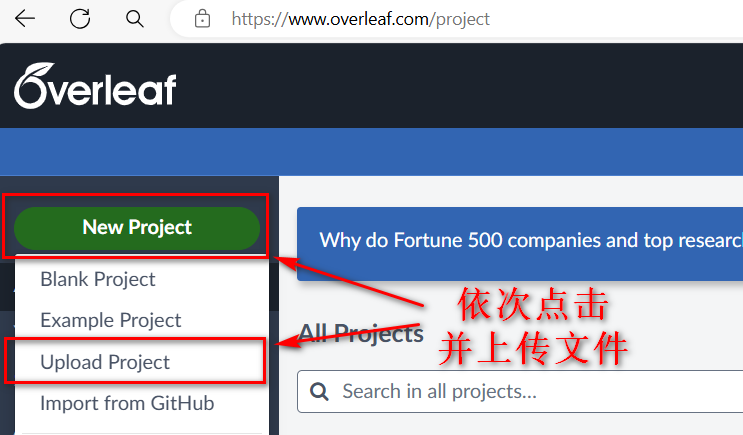
\includegraphics[width=\linewidth]{overleaf_0.png}
    \end{center}

    \item 在Windows系统的电脑上,打开C盘,搜索Fonts,找到该文件夹,然后将里面的simkai.ttf(楷体), simsun.ttf(宋体), times.ttc(Times New Roman), simhei.ttf(黑体),timesbd.ttf(Times New Roman bold)几种字体上传至Project的根目录/主文件夹下。

    如果不执行这一步操作,仍然可以使用,但是需要注意的是,因overleaf的系统为Ubuntu,字体与Windows系统下的字体略有差别。
    
    \item 点击菜单按钮,并将编译方式设置成xeLaTeX.
    \begin{center}
        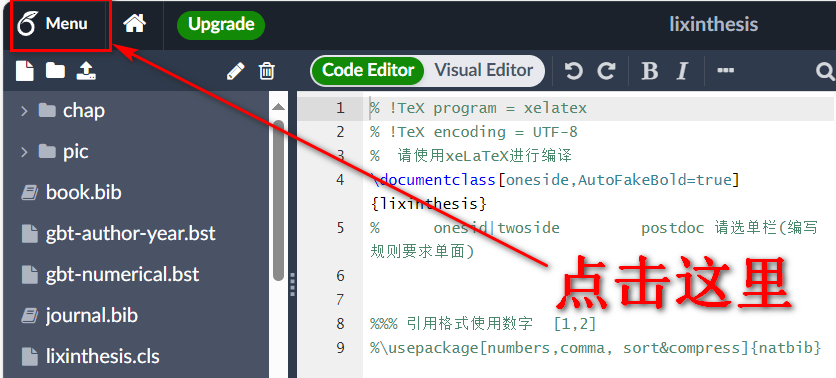
\includegraphics[width=0.65\linewidth]{overleaf_1.png}
        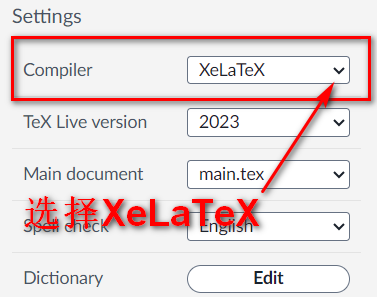
\includegraphics[width=0.3\linewidth]{overleaf_2.png}
    \end{center}
    \item 点击中间编译按钮,编译文件生成PDF文档。
    \begin{center}
        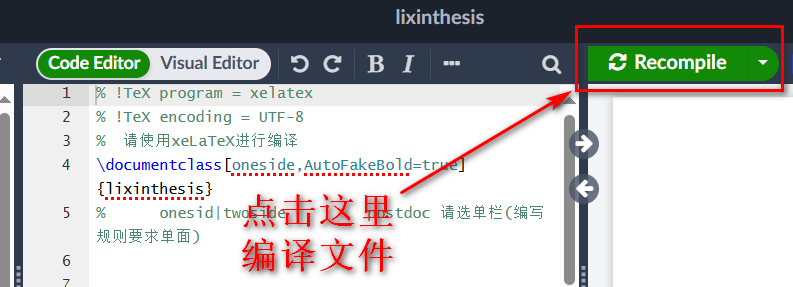
\includegraphics[width=\linewidth]{overleaf_3.png}
    \end{center}
\end{enumerate}



\backmatter %%%% 后文部分

\bibliography{bibref} %%% 参考文献
\begin{appendix}
附录在这里,这里可以放一些代码或者其它内容。
\begin{lstlisting}[caption=代码抄录示例,language=Matlab,label=code:exm2]
function s = f(x)
% This Program gives the area of a circle.
% S = F(x)
    pi = 3.14;
    
    s = pi*x^2;
end
\end{lstlisting}

\end{appendix}   %%%% 附录,不需要注释掉
\begin{thanks}
	致谢在这里
    
    
    \begin{flushright}
        致谢人:sslchi\\
        \the\year{} 年 \the\month{} 月 \the\day{} 日
    \end{flushright}
\end{thanks}     %%%% 致谢

\end{document}
